\documentclass[12pt,a4paper]{article}
\usepackage[utf8]{inputenc}
\usepackage[english]{babel}
\usepackage{amsmath}
\usepackage{amsfonts}
\usepackage{amssymb}

\usepackage{hyperref}

\usepackage{graphicx}
\graphicspath{ {./images/} }
\usepackage{epstopdf}

\usepackage[top=1.5in, bottom=1in, left=1in, right=1in]{geometry}


% alignment of figures (H)
\usepackage{float}

% tikz graphs
\usepackage{tikz}
\usetikzlibrary{arrows,automata, positioning,calc,shapes.geometric}
\usepackage{varwidth} % for the diagram of fpga design

\usepackage{todonotes}

% for tanles
\usepackage{multirow}

% header
\usepackage{fancyhdr}
\pagestyle{fancyplain}
\fancyhf{}
\lhead{ \fancyplain{}{Lukas Schwartz \& Aitor Miguel } }
\rhead{ \fancyplain{}{EMB1 - 1. Semester MSc Robot Systems} }
\cfoot{ \fancyplain{}{\thepage} }

% make tables prettyer
\def\arraystretch{1.3}

\begin{document}

\begin{titlepage}
	\centering
%	\includegraphics[width=0.15\textwidth]{example-image-1x1}\par\vspace{1cm}
	\vfill
	{\scshape\LARGE University of Southern Denmark\par}
	\vspace{1cm}
	{\scshape\Large EMB1 Project \#1\par}
	{\scshape\large 1. Semester MSc Robot Systems\par}
	\vspace{1.5cm}
	{\huge\bfseries Mini Segway\par}
	\vspace{2cm}
	{\Large\itshape Aitor Miguel Blanco \& Lukas Chr. M. W. Schwartz \\ Group \#1 \par}
	\vfill
	supervised by\par
	J\o rgen Christian Larsen \& Richard Beck

	\vspace{2cm}

% Bottom of the page
	{\large 23$^{rd}$ December 2015 \par}
\end{titlepage}

\pagebreak

\section*{Project Description}





what we need:

\begin{itemize}
\item 2 motors
\item accelerometer and gyroscope
\item FPGA (we have)
\item possibly ADC if analogue acc/gyro (we have)
\item motor driver (should be able to build ourself)
\end{itemize}

\pagebreak


\tableofcontents

\pagebreak

\listoffigures

\listoftables

\pagebreak



\section{Introduction}

This project describes the creation of an autonomous brick sorter to sort red, green and blue Lego bricks into separate directions.
This is to be done using a slide to which there is attached a servo motor to control whether the brick is going to the left or right.
Furthermore this project considers the design of the circuits used for power supplies and   color detecting circuit.

For the control of the brick sorter a FPGA is used to control the system.
The project also requires the use of uTosNet to communicate with a computer.

This report is structured such that it first describes the hardware and schematics used.
Thereafter the program run on the FPGA is considered and finally a test of the system is conducted and a conclusion on the whole project is drawn.



%This way, the project can be easily divided in 6 different blocks,

%\begin{itemize}
%\item Power supply
%\item Light sensor.
%\item LED Control.
%\item Servo motor.
%\item PC communication.
%\item VHDL design.
%\end{itemize}
	
\pagebreak


\section{Circuit and Physical Design}
To solve the sokoban problem a robot capable of performing simple tasks concerned with moving the can and itself around the game map are needed.
The behaviours the robot should be able to perform define how the robot should be formed in order to accomplish its task of solving the sokoban problem.


\subsection{Sensors}
In order to control and stabilize the Segway, then a set of sensors are required.
For this project it was decided to both use a set of sensors to control the systems stability and also to implement a set of sensors into the system enabling the tracking of the Segways position.


The tracking of the Segways position is done using an encoder kit\footnote{ \href{https://www.sparkfun.com/products/13339}{Wheel encoder}} mounted on the motors used in this project.
The encoders chosen for this project is an incremental rotary encoder capable to track the movement of the wheels, but not the direction of rotation.
It is hence not directly possible to tell which direction the Segway is moving without combining it with data from other sensors.
The sensors were however deemed good enough for the scope of this project.


The most important sensor of the system is the one used to control the stability of the system in order to hold it upright.
For this an accelerometer or/and a gyroscope can be used.
The advantage of using a gyroscope is that it is reliable in the measure of angular displacement over short periods of time.
When integrating over this it does, however, get troublesome due to drifts when performing the numerical integration.
The accelerometer on the other hand is exposed to a lot of noise from all the surrounding forces working on the system and it is hence only becomes a reliable measure of the systems angle when used with a low-pass filter.
It was therefore decided to use both in the project and combining them using a complimentary filter.
This provides the system with both the short term accuracy of the gyroscope and the long term reliability of the accelerometer.
For this project it was decided to by an integrated circuit
\footnote{ \href{https://www.sparkfun.com/products/13339}{IMU component}}
 including both gyroscope and accelerometer in the same component.
This ensures that the axis of the accelerometer and gyroscope are aligned within the component.





\subsection{Motor Control}
The motors chosen for this project were the two small geared DC motors\footnote{ \href{https://www.sparkfun.com/products/13258}{Motors}}.
In order to control them an H-bridge for both of the motors were constructed using the schematics in figure \ref{fig:hbridge}.


\begin{figure}[H]
\centering
%\includegraphics[width = 0.9 \textwidth]{•}

\caption{H-bridge schematics.}
\label{fig:hbridge}
\end{figure}

A full H-bridge is required in order to control the Segways movement in both directions such that it is able to both move and recover from a fall when moving around.
Each motor is made with each their separate H-bridge in order to facilitate the rotation of the segway.

\todo[inline]{write short about the h bridge design and different transistors used}


\subsection{The Segway System}
\todo[inline]{the combined system, all connected together}

\subsection{Conclusion}
A set of motors were chosen and for these a full H-bridge designed to be controlled by the output of the FPGA.
An IMU was also selected to use in order to control the inclination of the segway and keep it stable.
Furthermore a power supply was designed to convert the input voltage to the system into the required 5V range of the FPGA.

The set of components were then put together to form a segway with the main goal of distributing the weight evenly on the FPGA to  enhance its stability.

\pagebreak
\section{Software}
This section describes the software used to control the brick sorting system.
First the top module is described and from there the individual components are considered.

The main components and their interface is shown in figure \ref{fig:program_design}.
Apart from the shown connections in figure \ref{fig:program_design}, then a set of connections to transfer variables which can be set from the computer and the clock signal.


\begin{figure}[H]
\centering
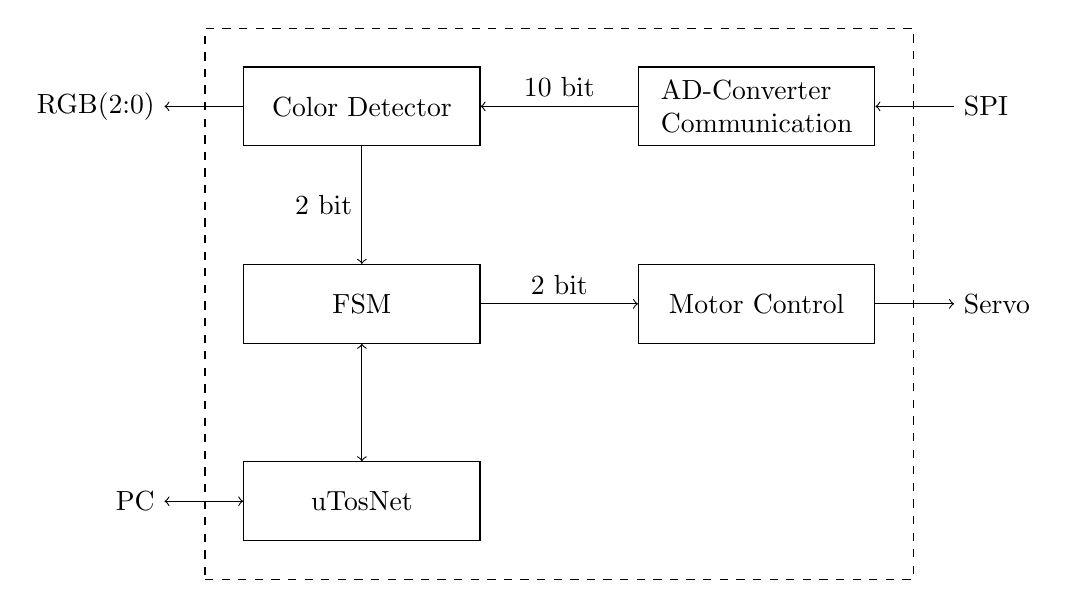
\begin{tikzpicture}[node distance=1cm]
% FPGA border
\node[rectangle,draw,minimum width=9cm, minimum height=7cm, dashed, name=FPGA]  {};

% used to align the insides of FPGA
\node[rectangle,minimum width=5cm, minimum height=5cm, name=FPGAaligne] {};

% components of FPGA
\node[rectangle,draw,minimum width=3cm, minimum height=1cm, name=utos] at (FPGAaligne.-135) {uTosNet};
\node[rectangle,draw,minimum width=3cm, minimum height=1cm, name=ad] at (FPGAaligne.45) {\begin{varwidth}{4cm}AD-Converter\\ Communication\end{varwidth}};
\node[rectangle,draw,minimum width=3cm, minimum height=1cm, name=mc] at (FPGAaligne.0) {Motor Control};
\node[rectangle,draw,minimum width=3cm, minimum height=1cm, name=fsm] at (FPGAaligne.180) {FSM};
\node[rectangle,draw,minimum width=3cm, minimum height=1cm, name=color] at (FPGAaligne.135) {Color Detector};

% nodes outside FPGA
\node [left=of utos,name=pc] {PC};
\node [right=of ad,name=adc] {SPI};
\node [left=of color,name=rgb] {RGB(2:0)};
\node [right=of mc,name=servo] {Servo};

% arrows inside FPGA
\draw[<->] (utos) -- node[] {} (fsm) ;
\draw[<-] (color) -- node[above] {10 bit} (ad) ;
\draw[->] (fsm) --  node[above] {2 bit} (mc) ;
\draw[->] (color) -- node[left] {2 bit} (fsm) ;
 
% arrows connected to the outside of FPGA
\draw[<->] (utos) to[out=180, in=0] node[] {} (pc) ;
\draw[->] (adc) to[out=180, in=0] node[] {} (ad) ;
\draw[->] (color) to[out=180, in=0] node[] {} (rgb) ;
\draw[->] (mc) to[out=0, in=180] node[] {} (servo) ;
\end{tikzpicture}

\caption{FPGA Program Design.}
\label{fig:program_design}
\end{figure}



The components of figure \ref{fig:program_design} are responsible for the following tasks.

\paragraph*{FSM}
The \textit{FSM} component is the top module of the system.
It connects the remaining components functionality in order to sort the bricks depending on their color and communicate with the computer.

\paragraph*{Color Detector}
The \textit{Color Detector} is responsible for controlling the LEDs and use the data from the ADC to decide the color of the bricks passing through the system.
This way it is able to connect the light intensity values from the photo-diode and relate them to a specific color.
From there the data is used to decide which brick, if any, is passing the sensor.

\paragraph*{AD-converter Communication}
This component implements the SPI communication to the ADC and feeds this onwards to the \textit{Color Detector}.


\paragraph*{Motor Control}
The \textit{Motor Control} component is controlling the servo motor using an input signal, deciding which of three positions it should be in.
Either the left- or right-tray or the idle position.

\paragraph*{uTosNet}
UTosNet is the component supplied by SDU which implements the communication with the computer.
This component is hence created such that it is capable of transferring data of importance to the FPGA and change specific settings or gather data from such.




\subsection{Segway Control}
The \textit{segway control} module is the top module of the design and in charge of the data transfer between the different underlying modules and the communication between the IMU.
It is implemented as the state machine seen in figure \ref{fig:segwaycontrol_fsm}.


\begin{figure}[H]
\centering

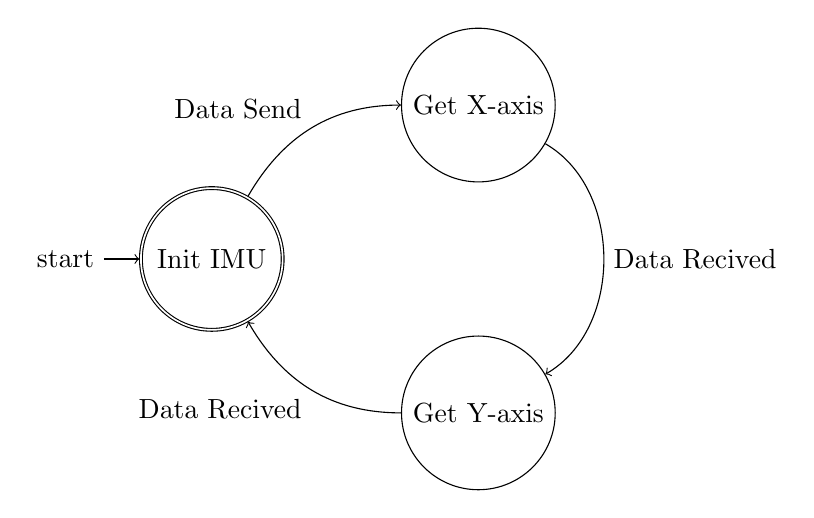
\begin{tikzpicture}[node distance=3cm]
\node[circle, minimum width=4.5cm, name=c] {};

% node circles
\node[initial,accepting,state,name=init,minimum width=1.8cm] at (c.180)   {Init IMU}; 
\node[state,name=xaxis,minimum width=1.8cm] at (c.60)   {Get X-axis}; 
\node[state,name=yaxis,minimum width=1.8cm] at (c.-60)   {Get Y-axis}; 

% connections
\draw[->] (init) to[out=60, in=180] node[midway,above left] {Data Send} (xaxis) ;
\draw[->] (xaxis) to[out=-30, in=30] node[midway,right] {Data Recived} (yaxis) ;
\draw[->] (yaxis) to[out=-180, in=-60] node[midway,below left] {Data Recived} (init) ;
 
\end{tikzpicture}

\caption{Finite state machine of the Segway Control module.}
\label{fig:segwaycontrol_fsm}
\end{figure}

The module is, as seen in figure \ref{fig:segwaycontrol_fsm}, looping between a set of states where it is communicating with the IMU.
In this design only acceleration of the robot in the frontal/backward direction (x-axis) is considered due to time constraints.
This is hence the only value stored and send onwards in the system.
The values of interest are requested in the state machine and then send to the \textit{filter} module for further processing.

In the state machine seen, the IMU is initiated every cycle.
This was done to ensure that the IMU has the right configuration when data is requested due to the possibility that a short power break shuts down the IMU and forces it into its default sleep mode.


\subsection{SPI Module}
To communicate with the IMU a SPI module was made.
The module is made up of three phases.
One being the phase where the slave is told what is going to happen.
The second being the read or write phase where the FPGA either reads data from the IMU or sends data to the IMU.
Finally there is the wait state where there is no communication amongst the two units.

The SPI module was implemented as an 8 bit data transmitter and receiver.
It is however possible to read multiple bytes in succession from the IMU, it was however deemed unnecessary to use all 16 bit the current version of the segway.
\subsection{Data Filter}

The value in an accelerometer is often noisy.
In our case the noise largely originates from motor vibrations and the acceleration caused by the general movement of the segway.
This can give problems in cases where small movements of the device are important and in general if big noise spikes are encountered.
To solve this problem, the commonly used solution is to combine the value given by the gyroscope with that of the accelerometer readings to obtain a more accurate prediction of the angle.
As this approach is complex and not really needed to obtain a simple control of the segway, a more simple solution was selected.

The accelerometer data is filtered using a mean filter to reduce high frequency noise form the motor vibrations.
The filtering module calculates the mean of the last eight readings from the accelerometer, outputting a 8 bit value.
These 8 bits represent the value of acceleration obtained, being 0 m/s$^{2}$ the value 127, all the values above it positive and all the values below negative.
This filter module is also used to converter the data from the accelerometers format into this new data representation going from negative acceleration at 0 to positive acceleration at 256 and zero acceleration at 127.
\subsection{PID Controller}

The PID module developed implements a PID controller using as a input a reference signal for the desired value of the accelerometer and the actual acceleration value as two logic vectors.

As all the operations in the PID are calculated using integers, then the data vectors are converted into integers before the operations and reconverted into a logic vector afterwards.
%The  again representing the value of the duty cycle needed in the motors and their direction.
The output vector generated is a 9 bit signal.
The eight least significant bits representing the chosen duty cycle and the most significant bit the direction of the motors, that is positive for forward and negative backwards.

Three different values can then be set to modify the PID performance.
The gain for the proportional, integral and differential part.

\subsection{Motor Control}
The Motor control unit controls the input to the eight different inputs on the two H-bridges.
This control was implemented as the finite state machine seen in figure \ref{fig:motorcontrol_fsm}.

The main purpose of the motor control unit is to set two of the ports of the motor low and the two others high depending on the direction the segway is moving.
When controlling the speed a PWM signal is send to one of the ports of the H-bridge to control the speed depending on the value calculated in the PID controller.


\begin{figure}[H]
\centering

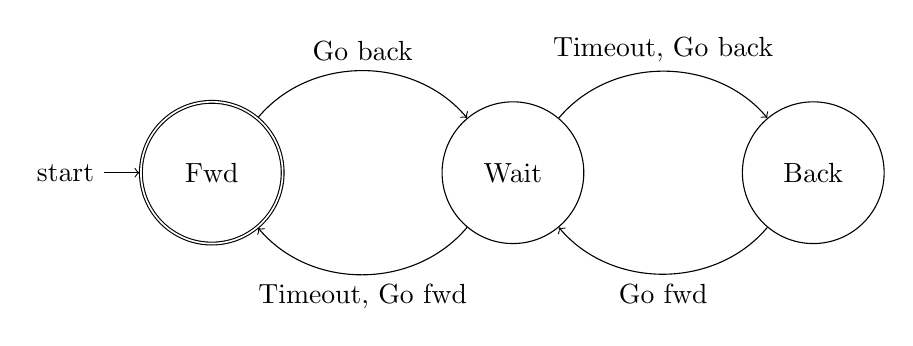
\begin{tikzpicture}[node distance=2cm]

% node circles
\node[initial,accepting,state,name=fwd,minimum width=1.8cm] {Fwd}; 
\node[state,name=wait,minimum width=1.8cm, right=of fwd] {Wait}; 
\node[state,name=back,minimum width=1.8cm, right=of wait] {Back}; 

% connections
\draw[->] (fwd) to[out=50, in=130] node[midway,above] {Go back} (wait) ;
\draw[->] (wait) to[out=50, in=130] node[midway,above] {Timeout, Go back} (back) ;
\draw[<-] (fwd) to[out=-50, in=-130] node[midway,below] {Timeout, Go fwd} (wait) ;
\draw[<-] (wait) to[out=-50, in=-130] node[midway,below] {Go fwd} (back) ;
 
\end{tikzpicture}

\caption{Finite state machine of the Motor Control module.}
\label{fig:motorcontrol_fsm}
\end{figure}


As seen on figure \ref{fig:motorcontrol_fsm}, then a wait state is put between the two driving states, forward and backward.
This was done to protect the motor when switching between the states.
It is necessary to have a delay because of the turn of and turn on delays of the transistors.
If this is not set it may result in all the transistors being open at once and thus damaging the motor.
The delay was set to 160ns which is considerably more than the turn on and turn of delay of the transistors, but small enough that it should not be noticed when driving the motors.
During this time all the transistors are set off.

The PWM generated at the motors is based on a 8 bit signal and there are hence 256 different duty cycles to drive the motors with.

\subsection{Conclusion}
An A* algorithm was devised to solve the Sokoban problem.
The algorithm uses a graph structure where the nodes represent diamond pushes with the cost being the number of steps the robot must move in order to achieve the state.

The heuristic for the A* algorithm was found calculating the cost for the robot to move each diamond from their current position to the nearest goal.
This technique takes into account the walls on the map, but disregard the diamonds left on the map disrupting the path.
Furthermore the cost of moving in between the diamonds and the fact that one goal may be considered the destination of multiple diamonds is not taken into account using this method.

The nodes in the graph where also validated using their state, in form of the diamonds and robots position, as the key in a hashing table.
Furthermore the states are checked for simple deadlock situations.





\pagebreak
\section{Test of the System}
The final system was tested to see how well it performs.
The tests where performed in normal ambient light and with the thresholds set beforehand to a suitable value.

A set of bricks where let slide through the setup and the result shown in the confusion table in table \ref{tab:confusiontable_testresults}.


\begin{table}[H]
\centering
\begin{tabular}{|c|c|c|c|c|}
\hline
 & &  \multicolumn{3}{|c|}{Predicted} \\ \hline
 & & Red & Green & Blue \\ \cline{1-5} 
\multirow{3}{*}{Actual} & Red & & & \\ \cline{2-5}
 & Green & & & \\ \cline{2-5}
 & Blue & & & \\ \hline
\end{tabular}
\caption{Confusion table of the test results.}
\label{tab:confusiontable_testresults}
\end{table}

\pagebreak
\section{Conclusion}

After building the robot and testing all the implemented behaviours, it was found that the proposed solution is robust enough to execute any given path.
The robot works under different ambient light levels due to a mounted shield that shadows the sensors, making them less sensitive to external light.
The robot can run for over 30 minutes without problems from having a low battery level.

To find a solution for the Sokoban problem an A* algorithm has been devised.
Using the diamond pushes as nodes and the number of steps of the robot to achieve a certain state as the cost.
The algorithm uses, as heuristics, the cost of moving each diamond from their position to the nearest goal when having to push them around the walls in a else completely empty map.
The nodes in the graph are validated using the diamonds and robots state.
The individual states are checked for deadlock situations to reduce the graph.

The solver can work for any map satisfying a constrained map size.

To load the generated path into the robot, a path converter was implemented.
This function can convert the generated path to be executable for the robot.

By combining the two parts of this project, it is possible to load a certain sokoban map, find a solution for it and solve physically the challenge with the robot.


\pagebreak
\section{Discussion}
The segway constructed has a physical design of such that it is deemed good enough.
The only changes which should be made are replacements of the connectors which should be updated to give a more reliable connection to the motors and from the power supply to the H-bridge.

Since the system was not able to balance itself, then it is probably the software system that is needing the biggest upgrade.
This includes going away from only using only one axis of the accelerometer and trying to set its the gravitational effect of such to zero.
To possibly using two axis of the accelerometer to predict the actual angle of the segway.
This would require the implementation of the 'atan' function on the FPGA.
Given that the current FPGA used only has 54k bits of block RAM, then this implementation has to be an approximation of the function since not enough space is present for a direct table lookup.

Given that a successful implementation of the calculation of the angle of the segway has been found, then this can also be combined with the gyroscope data.
This can then be used to implement a complimentary filter, Kalman filter or similar.

It is furthermore possible to investigating other controller options to improve the performance of the segway or use different controllers when in different situations.
That is having different PID controllers when the segways incline is within a certain range.

Once the segway is able to stand by itself it would also be of interest to make it possible to control it through the bluetooth device.
The encoders could then be used to control its odometry of the segway to turn it and drive it around a specific speeds.

\pagebreak
\appendix




\end{document}